\documentclass[10pt,twocolumn,openany,nodeprecatedcode,bg=none]{dndbook}

\usepackage[english]{babel}
\usepackage[utf8]{inputenc}
\usepackage{graphicx}

% Don't skip an extra page before mainmatter.
\makeatletter
\renewcommand\mainmatter{\clearpage\@mainmattertrue\pagenumbering{arabic}}
\makeatother

\DndSetThemeColor[DmgSlateGray]

\title{A First Encounter}

\begin{document}

\frontmatter%

\tableofcontents

\nopagebreak
\mainmatter%

\chapter{Creatures}
The creatures encountered in this adventure.

\section{Regular}
These creatures are as seen in the monster manual.

\begin{DndMonster}[width=\textwidth]{Goblin}
\begin{multicols}{2}
  \DndMonsterType{Small humanoid (goblinoid), neutral evil}
  \DndMonsterBasics[
    armor-class=15,
    hit-points=\DndDice{2d6},
    speed=30 ft.
  ]
  \DndMonsterAbilityScores[str=8, dex=14, con=10, int=10, wis=8, cha=8]
  \DndMonsterDetails[
    skills={Stealth +6},
    senses={Darkvision 60ft., passive Perception 9},
    languages={Common, Goblin},
    challenge={1/4}
  ]
  
  \DndMonsterAction{Nimble Escape}
  The goblin can take the Disengage or Hide action as a bonus action on each of its turns.

  \DndMonsterSection{Actions}
  \DndMonsterMelee[
    name=Scimitar,
    mod=+4,
    reach=5,
    targets=one target,
    dmg=\DndDice{1d6+2},
    dmg-type=piercing
  ]
  \DndMonsterRanged[
    name=Shortbow,
    mod=+4,
    range=80/320,
    targets=one target,
    dmg=\DndDice{1d6+2},
    dmg-type=piercing
  ]
\end{multicols}
\end{DndMonster}

\begin{DndMonster}[width=\textwidth]{Bugbear}
\begin{multicols}{2}
  \DndMonsterType{Medium humanoid (goblinoid), chaotic evil}
  \DndMonsterBasics[
    armor-class=16,
    hit-points=\DndDice{5d8+5},
    speed=30 ft.
  ]
  \DndMonsterAbilityScores[str=15, dex=14, con=13, int=8, wis=11, cha=9]
  \DndMonsterDetails[
    skills={Stealth +6, Survival +2},
    senses={Darkvision 60 ft., passive Perception 10},
    languages={Common, Goblin},
    challenge={1}
  ]
  
  \DndMonsterAction{Brute}
  A melee weapon deals one extra die of its damage when the bugbear hits with it (included in the attack).

  \DndMonsterAction{Surprise Attack}
  If the bugbear surprises a creatue and hits it with an attack during the first round of comabt, the target takes an extra \DndDice{2d6} damage from the attack.

  \DndMonsterSection{Actions}
  \DndMonsterMelee[
    name=Morningstar,
    mod=+4,
    reach=5,
    targets=one target,
    dmg=\DndDice{1d6+2},
    dmg-type=piercing
  ]
  \DndMonsterMelee[
    name=Javelin,
    mod=+4,
    reach=5,
    targets=one target,
    dmg=\DndDice{2d6+2},
    dmg-type=piercing
  ]
  \DndMonsterRanged[
    name=Javelin,
    mod=+4,
    range=30/120,
    targets=one target,
    dmg=\DndDice{1d6+2},
    dmg-type=piercing
  ]
\end{multicols}
\end{DndMonster}

\section{Unique}
These monsters were created for this adventure.

\begin{DndMonster}[width=\textwidth]{Goblin Priest}
\begin{multicols}{2}
  \DndMonsterType{Small humanoid (goblinoid), neutral evil}
  \DndMonsterBasics[
    armor-class=12,
    hit-points=\DndDice{2d6},
    speed=30 ft.
  ]
  \DndMonsterAbilityScores[str=8, dex=8, con=10, int=10, wis=14, cha=12]
  \DndMonsterDetails[
    skills={Stealth +6},
    senses={Darkvision 60ft., passive Perception 12},
    languages={Common, Goblin},
    challenge={1/4}
  ]
  
  \DndMonsterAction{Spellcasting}
  The goblin priest is a 1\textsuperscript{st} level spellcaster.
  Its spellcasting ability is Wisdom (spell save DC 12, +4 to hit with spell attacks).
  The goblin priest has the following cleric spells prepared:
  \begin{DndMonsterSpells}
    \DndMonsterSpellLevel{Thaumaturgy, Sacred Flame, Light}
    \DndMonsterSpellLevel[1][2]{Command, Cure Wounds, Healing Word}
  \end{DndMonsterSpells}

  \DndMonsterSection{Actions}
  \DndMonsterMelee[
    name=Mace,
    mod=+0,
    reach=5,
    targets=one target,
    dmg=\DndDice{1d6-1},
    dmg-type=bludgeoning
  ]
\end{multicols}
\end{DndMonster}

\chapter{Areas}
The areas found in this adventure.

\DndArea{Town of Falbright}
\begin{DndReadAloud}
  It is late afternoon as you approach the town of Falbright, as noted on a waypost some time ago in your journey.
  It looks to be a town of 20-30 people, located on a secondary trade route in the province of Darston.
  You pass one of the duke's roaming patrols as you enter, noticing that the buildings in town look well kept and maintained.
  There is a reasonably large inn, a blacksmith and general goods store combination, and a small church for the town's inhabitants serving the believers of good-aligned gods.
  You head towards the inn where you will be spending the night.
\end{DndReadAloud}

Players should be allowed to visit any of the church, blacksmith, or general goods store but should know they want to rest up to continue their journey tomorrow.

\DndSubArea{The Inn of the Dancing Pumpkin}
The Dancing Pumpkin is a family owned business -- father Geoffrey, mother Arion, son Simon.

Geoffrey is of slightly above average height fairly well muscled arms that say he probably cut all of the large pile of wood outside the inn and leaning near the fireplace inside.
He has short raven black hair over a well-wrinkled face.
If questioned about his obviously muscled build, he will mention his time spent in the duke's army and his decision to retire to raise his family with his wife.

Arion is also of slightly above average height and pregnant with a second child.
Her hair is a dirty blonde.

Simon has shaggy hair colored a shade slightly darker than his mother's.

\DndSubArea{The Blacksmith and General Store}
At the blacksmith, players will find the blacksmith Winnifred -- Winny for short -- and her husband Alfred who runs the attached general goods store.
Winny is woman of average height and stocky build, auburn hair in a single short braid who appears gruff in initial conversation but clearly has a soft spot for her dear husband.
Alfred is a short, rotund, and balding man with a hearty laugh, a quick wit and a clear affection for his wife.

\subparagraph{Inventory}
Both establishments have no unusual items nor equipment.
The blacksmith may be convinced to do a rush job on simple equipment but it will not be available before the morning (i.e. after this adventure is complete).

\DndArea{The Boar Forest}
A thickly wooded forest on top of gentle hills.
There is a slight scent of pine overridden by the damp smell of deep forest.

Players will have to spend the night in the forest.
The dungeon master may choose to roll for a random encounter but can also choose to say the night passes uneventfully.

\DndSubArea{The Clearing}
\begin{DndReadAloud}
  You see a clearing containing a slow rise to a central hill.
  Three sides of the hill have moss-covered steps leading up to a large mausoleum.
  In the past this was probably a beautifully crafted resting place, but now that some of the roof has crumbled and a pillar or two have fallen to the ground, it looks a little ramshackle.
\end{DndReadAloud}

With a DC 12 Wisdom (Perception) check, players notice two goblin guards standing in the shadows of pillars next to the entrance of the mausoleum.

\subparagraph{Goblin patrol}
If the players choose to wait and watch the mausoleum they should encounter a patrol of two goblins.
Roll passive perceptions to check who sees who.

The guards at the entrance are being lazy and do not expect anyone to get past the patrol.
They should not be allowed to notice the combat if the goblin patrol is killed.

If one of the patrol members dies or is severely injured, the other should make a break for the clearing.
Decide based on how far they get what the effect on the guards is: may still not notice or may have heard something and now are on alert.

\DndArea{Tomb of The Circle of the Blessed}
The tomb of a long dead order of knights who died together in combat.
Its ruins stand atop a hill in the center of a clearing.

\DndSubArea{Guarded Entrance}
Two goblin are guarding the entrance; neither are being particularly stealthy nor are they being particularly observant.
Players may sneak up on them from behind.

If combat goes for more than two rounds and one of the goblins is severely injured or dead, the second goblin will attempt to retreat to the bivouac to alert the others.

\begin{DndReadAloud}
  The smell of feces, rotten food, and dirty bodies wafts from the entrance.
  You see worn and cracked marble stairs descending into darkness.
\end{DndReadAloud}

Dwarven inscription above the door reads ``Here lies the Circle of the Blessed''.

\DndSubArea{Goblin Bivouac}
Goblins have made their home here.
Tattered bed rolls and burnt out cookfires scatter the area.

The following number of goblins should be present in the room, regardless of whether or not one of the guards retreated to warn them:
\begin{table}[ht]
  \begin{DndTable}[width=\linewidth,header=Bivouac Encounter]{lX}
    \textbf{Players} & \textbf{Goblins}\\
    5 & 4 \\
    4 & 3 \\
    3 & 2
  \end{DndTable}
\end{table}

If a goblin has alerted them, they should be in fighting formation and prepared to fight.
The goblin who retreated should be near the entrance of the room.
It is likely that one goblin will have overturned a table and is taking cover behind it and has prepared a shot.

If they have not been alerted, the goblins are spread around the room and may be caught by surprise if the party does not use torches.
If the party is using torches, the goblins will be rushing to get set up but will not have any prepared actions.

As one or two goblins are left, if the goblin patrol was not encountered, two goblins should enter from behind the staircase.

All goblins should stand and fight: they will not retreat for fear of interrupting the priest's ritual.

\DndSubArea{The Circle of the Blessed Tribute Room}
There is a brazier in the middle of the room, a DC 8 Intelligence (History) check notes that this is for tributes made to the dead.
Directly across from the entrance is a heavy door on well oiled hinges.

\begin{DndReadAloud}
  The walls have been covered in an exquisitely detailed mosaic, though sheen has been dulled by the goblin cookfires.
  Sharp blues and greens, reds and yellows depict several scenes.

  First, a group of seven adventurers of together with various weapons outsretched, looked over by a glowing being.

  Next, the group holding back a chaotic melee of gruesome creatures and a cruel, chaotic-feeling form made of shadows.
  Behind them, a terrified group of dwarves.

  The final scene shows the group, all mortally wounded, and their enemies vanquished.
  The dwarves are crying over their protectors.
\end{DndReadAloud}

Further investigation shows this text above the first mosaic:
\begin{DndReadAloud}
  In Dwarven: ``To the Blessed Circle I am pledged and the downtrodden I will protect!''
\end{DndReadAloud}

Close investigation of the leader's belt in the first 

Opening the door on the far side reveals a passageway with some very dim light and the sound of distant chanting.

\DndSubArea{Scythe Trap}
DC 13 Wisdom (Perception) check will discover the trap.
DC 10 Dexterity (Thieves' Tools) will disable the trap.

Upon activating the trap make an attack roll (+3) with damage \DndDice{1d6} on hit.

\DndSubArea{The Priest and Guard}
The priest and its guard will have heard none of the combat from the previous room due to the heavy door.
The trap likewise is quiet enough that the priest and guard would not hear it if it were triggered.

The guard should see torchlight coming down the hall and advance to the doorway saying in goblin ``Leave! You shouldn't be here! You'll disturb him!''

During combat, if a player goes down and the bugbear is close to death, the bugbear should offer them the chance to take their friend and leave and never return.
If players take a long rest after rescuing their friend, they should return to find the goblins missing and Simon brutally sacrificed.

\DndSubArea{The Statue Room}
The room is dimly lit (unless the party has a torch) until the final enemy dies.
Those with darkvision see Simon, naked and dirty, laying still in cage in the back right of the room.

\begin{DndReadAloud}
  As you slay the final enemy, magical lights flare to life along the walls, brightly lighting the room.
\end{DndReadAloud}

Simon has a pulse but cannot be woken up without a long rest.

\DndSubArea{The Statue of Arvic}
Anyone who approaches the statue should see these glowing words:
\begin{DndReadAloud}
  In Dwarven: ``If you are to keep this, you must first give it to me''.
\end{DndReadAloud}

\DndSubArea{Secret Door}
DC 15 Intelligence (Investigation) or Wisdom (Perception) check discovers a strangeness along the wall where the secret door is.
Subtle scratches on the floor, the wall being a ever-so-slightly different shade, missing mortar between bricks where the hinge is.

DC 17 Intelligence (Investigation) or Wisdom (Perception) is sure there is a door here but are unsure how to open it.

DC 20 Dexterity (Thieves' Tools) can open the door without solving the riddle.

\DndSubArea{The Crypt}
The seven coffins of the Circle members are arrayed in this room with Arvic's on another slightly raised dais.
None of the coffins will open except Arvic's.

\DndSubArea{The Coffin of Arvic}
If Arvic's is opened, players should see a sword with a slight sheen on it.
When the sword is touched, a magical barrier should block the door and several of the coffins should open, releasing skeletons.

\begin{figure*}[h]
  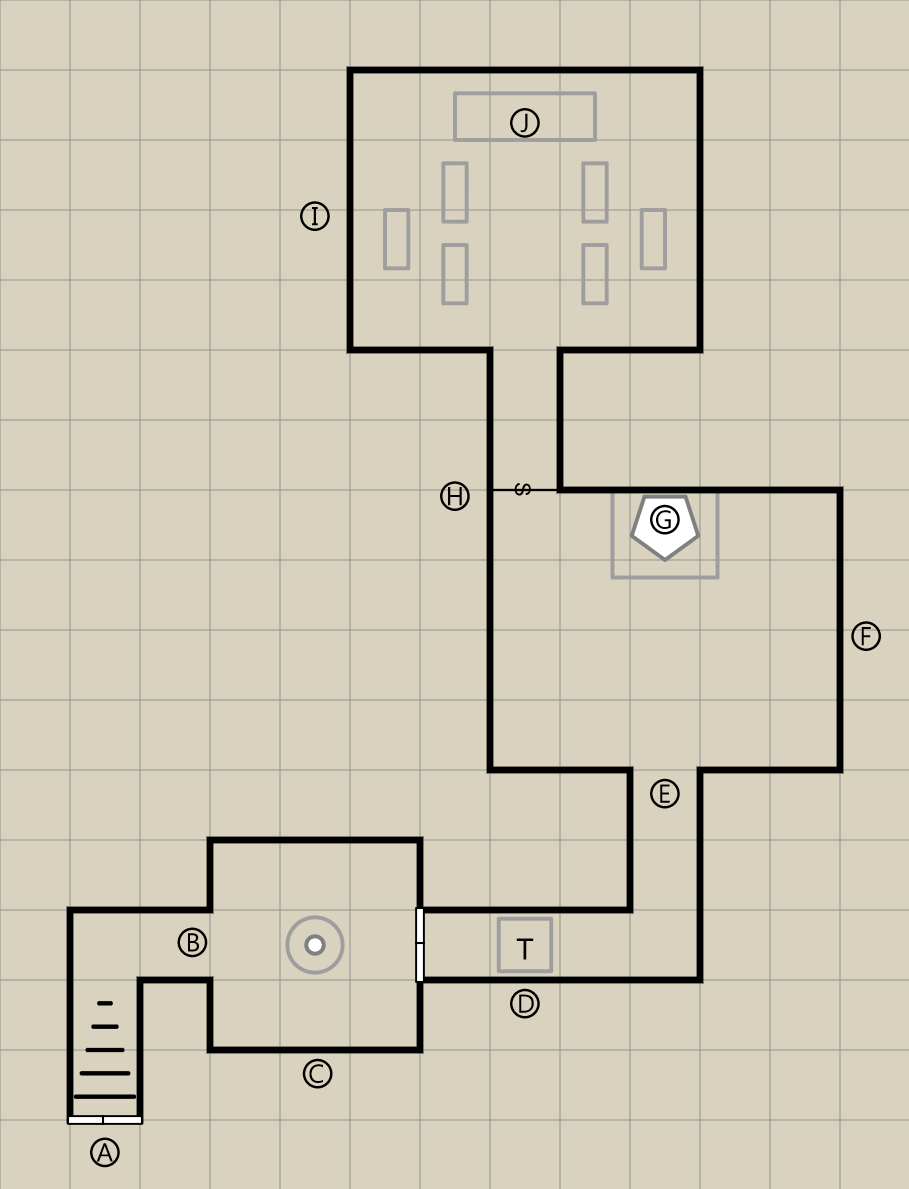
\includegraphics[height=.75\textheight]{assets/tomb.png}
\end{figure*}

\end{document}
